% Official contribution: https://conferences.iaea.org/event/498/contributions/43627/
% Scheduled date: 2026-10-28.
\paragraph{Abstract}
The Evaluated Nuclear Structure Data File (ENSDF)~\cite{ENSDF_Manual} is a foundational resource for nuclear structure
and decay information, providing evaluated data that support research across nuclear physics, nuclear energy, astrophysics, medicine, and national security. As experimental measurements continue
to grow in volume and complexity, new approaches are needed to improve both access to ENSDF and the efficiency of the evaluation process. The National Nuclear Data Center (NNDC) at Brookhaven National Laboratory is pursuing these goals through the modernization of ENSDF data services and the use of physics-informed artificial intelligence in nuclear data evaluation. 
\begin{figure}[htbp]
    \centering  
    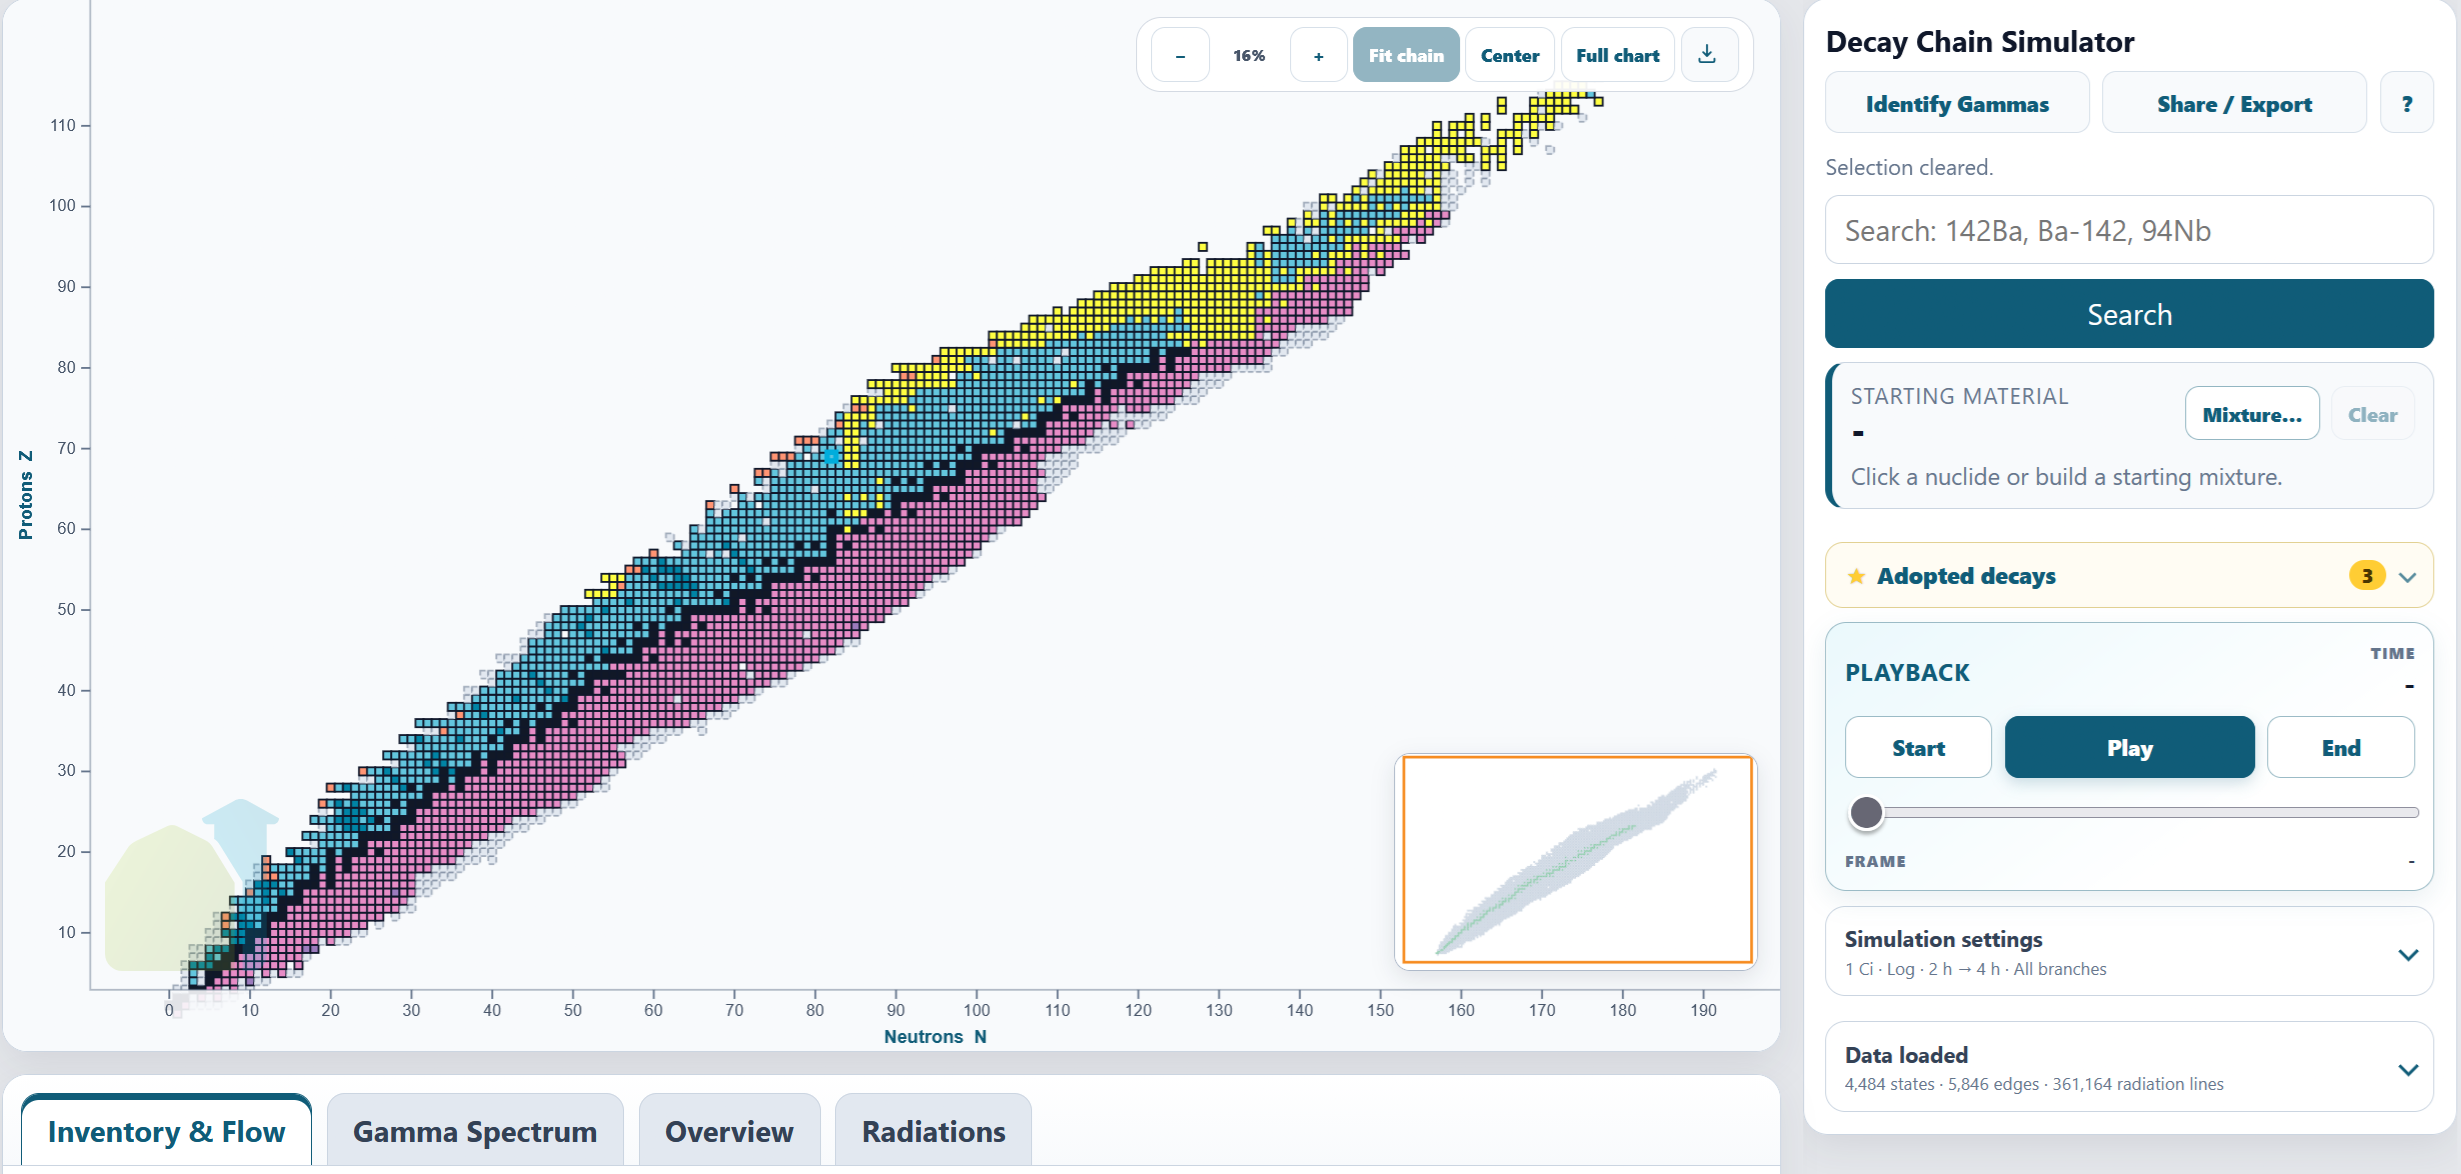
\includegraphics[width=.9\textwidth]{figures/mason_ss_1.png}
    \caption{Decay chain simulator featuring interactive chart of nuclides}
    \label{fig:submission_form}
\end{figure}
This talk will introduce the new ENSDF REST API~\cite{ensdf_api}, which provides standardized, programmatic access to evaluated nuclear structure and decay data and is publicly available at \url{https://www.nndc.bnl.gov/ensdf-api/}. The API makes ENSDF available to modern
scientific workflows, analysis software, web applications, and computational tools, and provides a foundation for new applications built around evaluated nuclear data.
With the addition of modernized access to nuclear data, interactive web applications are being developed. 
\begin{figure}[htbp]
    \centering  
    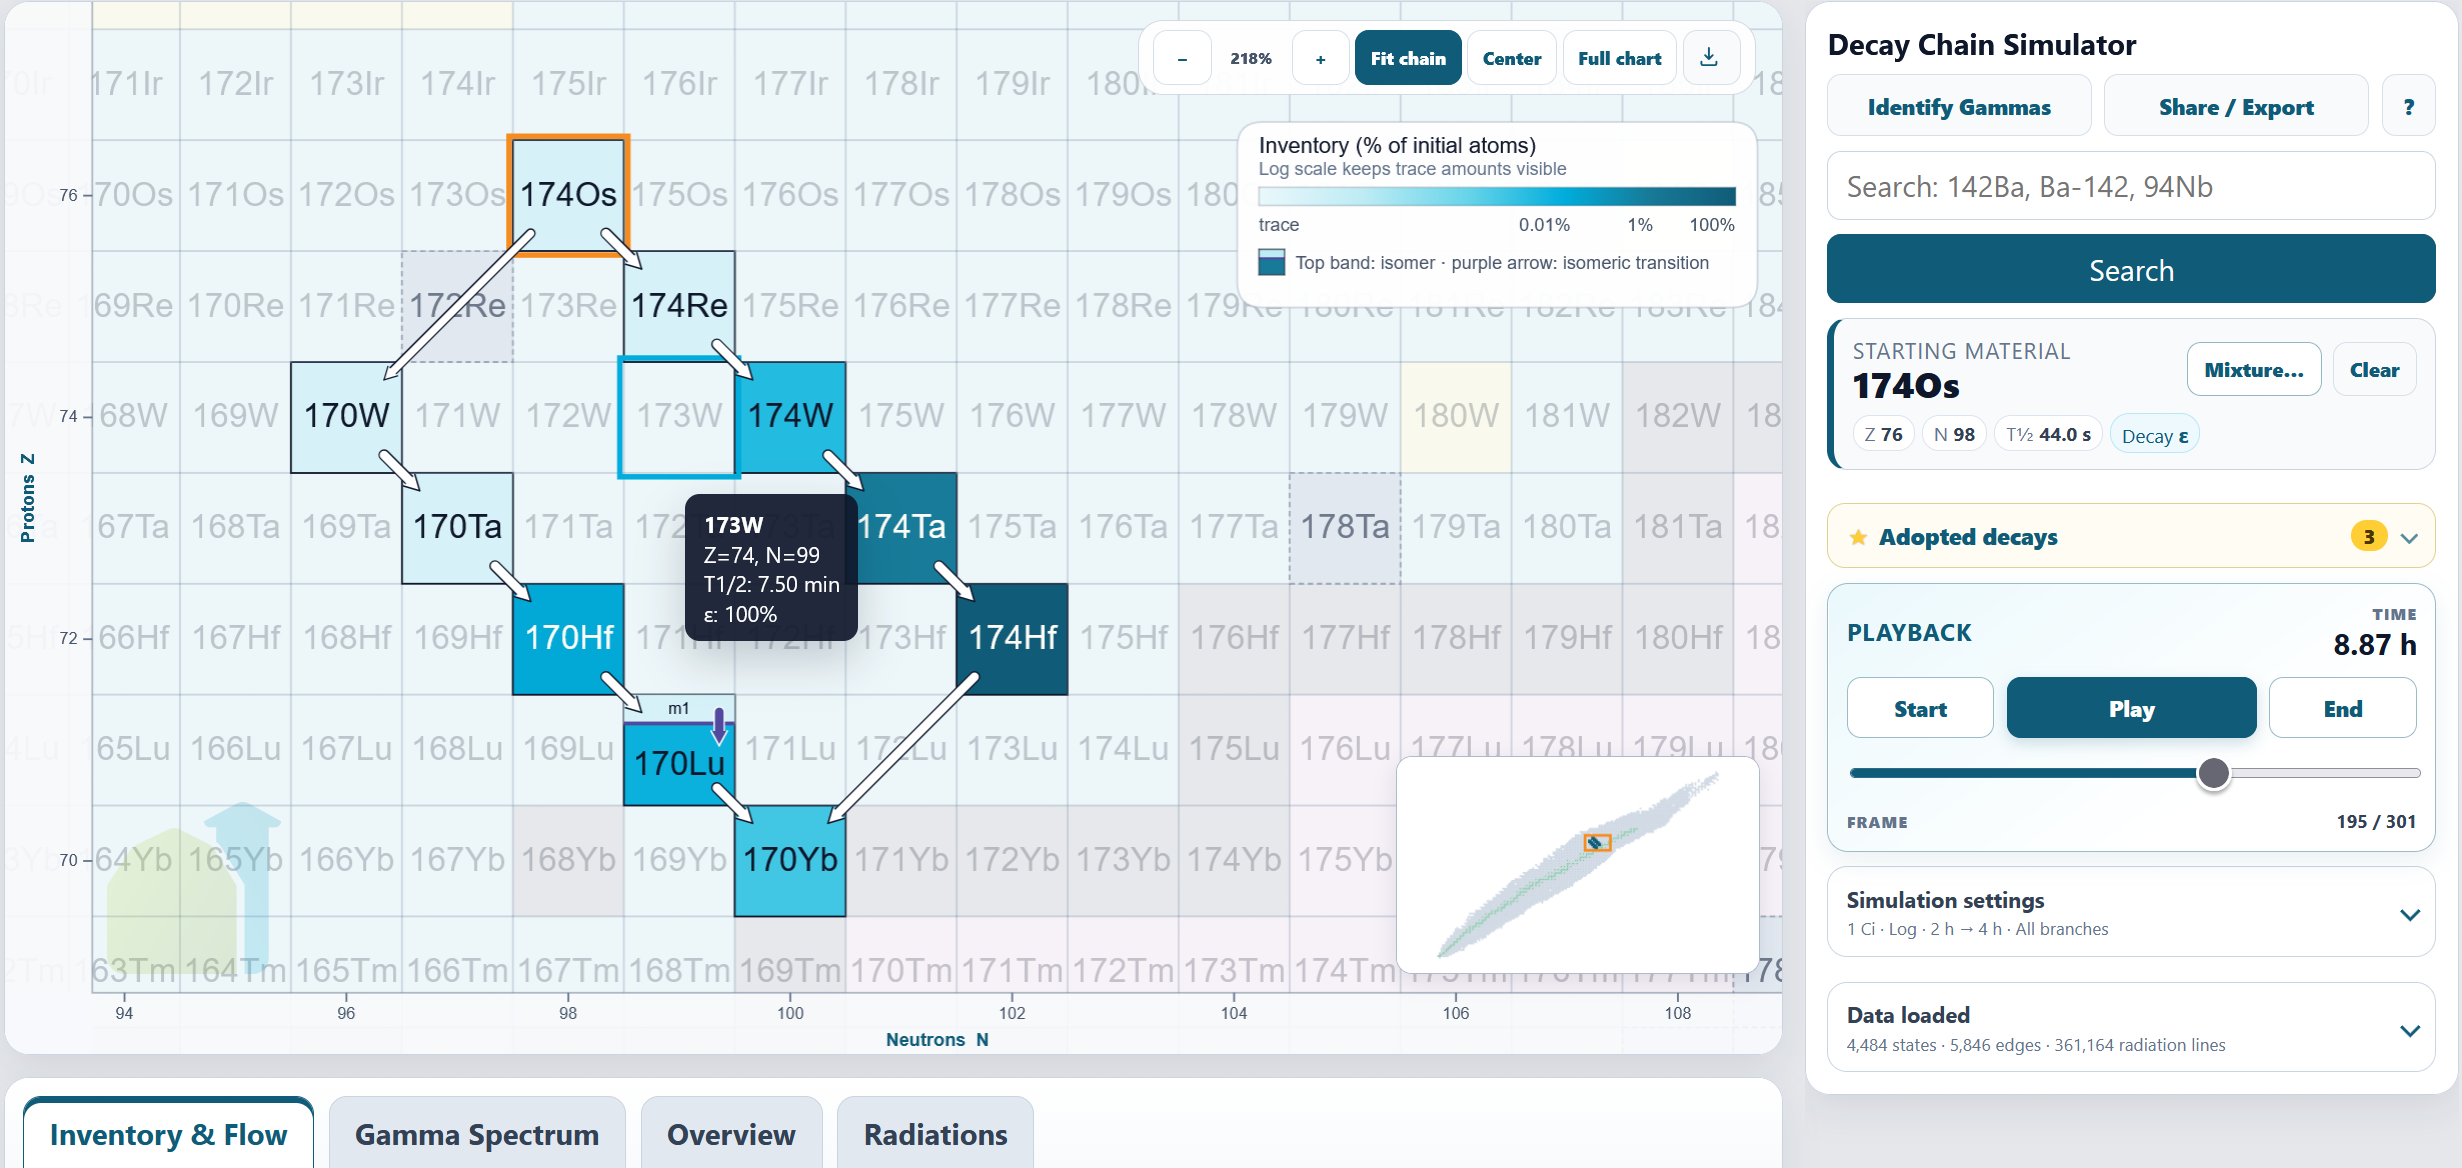
\includegraphics[width=.9\textwidth]{figures/mason_ss_2.png}
    \caption{Selecting a nuclide displays the entire chain and time controls are used to visualize the inventory over time.}
    \label{fig:submission_form}
\end{figure}
As part of the Adopted Decay project, we have implemented an interactive decay chain simulator.
The talk will also describe a newly funded effort supported through the U.S. Department of Energy’s Genesis Mission, a national initiative focused on using artificial intelligence to accelerate scientific
discovery. As part of this effort, the NNDC is investigating the use of physics-informed AI to assist with ENSDF evaluations while retaining expert oversight and the provenance and traceability required for evaluated nuclear data.
Four initial tasks have been identified: measurement reconciliation, using inference to compare
experimental measurements and determine consistent adopted values; J$\pi$  assignment, using classification to assist with nuclear spin and parity assignments; multipolarity assignment, using experimental observables and nuclear-structure information to identify transition multipolarities; and
anomaly detection, identifying unusual or potentially inconsistent data for further investigation by
evaluators.
Together, the ENSDF REST API and the Genesis Mission AI effort provide complementary approaches to modernizing ENSDF. The API provides programmatic access to the evaluated data, while the AI effort explores ways to make the evaluation process more efficient and help evaluators
handle increasingly large and complex datasets.
\begin{figure}[htbp]
    \centering  
    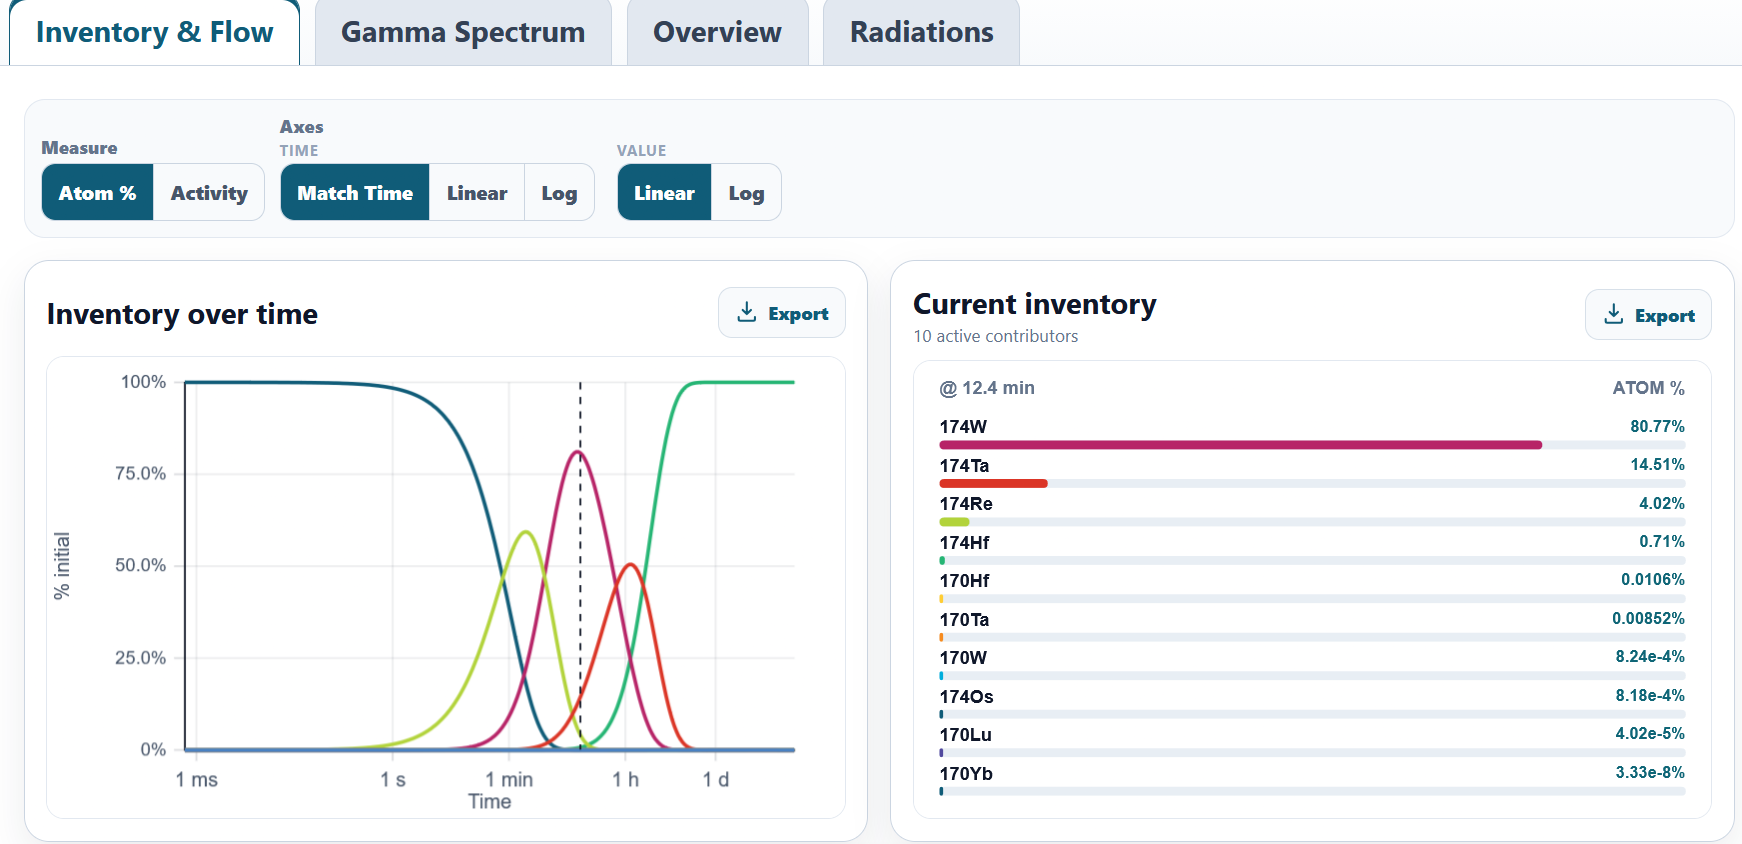
\includegraphics[width=.9\textwidth]{figures/mason_ss_3.png}
    \caption{Addition plots tracking inventory over time, current inventory, and even gamma spectra is provided.}
    \label{fig:submission_form}
\end{figure}


\paragraph{Discussion}
Donnie Mason presented REST APIs for NNDC databases. The APIs for ENSDF, ENDF and CapGam APIs are available now, and NuDat and Wallet Cards APIs are coming soon. He overviewed the Adopted Decay web application to simulated ENSDF decay data directly in a browser. Discussion covered selective retrieval, evaluation cutoff dates, and the provenance of adopted datasets. Mason then described the Genesis Mission project (St. Joseph’s University and BNL), which is developing physics-informed AI for four parts of evaluation: recommended values, multipolarities, spin-parity and anomaly detection. The approach is that AI proposes, deterministic tools decide, and evaluators make the final call. Schema references, explicit uncertainty representations, and reusable computational functions were discussed as further improvements.


